% Preambulo compartido para clases en formato beamer
\documentclass[9pt, xcolor=svgnames]{beamer}
\usepackage[utf8]{inputenc}
\usepackage[T1]{fontenc}
\usepackage[spanish,es-nodecimaldot]{babel}

\usetheme[progressbar=frametitle]{metropolis}
\metroset{sectionpage=none, subsectionpage=none}
\usepackage{appendixnumberbeamer}
\usepackage{booktabs}
\usepackage{amsmath,amssymb,bm,mathtools}
\usepackage{physics}
\usepackage{graphicx}
\usepackage{multicol}
\usepackage{tikz}
\usepackage{minted}
\usemintedstyle{tango}
\setminted{fontsize=\scriptsize, breaklines=true, linenos=true, bgcolor=LightGray!20, frame=lines}
\newminted{python}{fontsize=\scriptsize, breaklines=true, linenos=true, bgcolor=LightGray!20, frame=lines}
\usepackage{pgfplots}
\pgfplotsset{compat=1.18}
\usepackage{ragged2e}
\usepackage{xspace}
\newcommand{\themename}{\textbf{\textsc{metropolis}}\xspace}

\setbeamercolor{block title}{bg=MidnightBlue!85, fg=white}
\setbeamercolor{block body}{bg=MidnightBlue!5, fg=black}
\setbeamercolor{alerted text}{fg=Crimson}
\setbeamercolor{frametitle}{bg=MidnightBlue!10, fg=black}
\setbeamertemplate{blocks}[rounded][shadow=true]


\weektitle{06}{Algoritmo de Metropolis y modelo de Ising}

\begin{document}

\frame{\titlepage}

\begin{frame}{Organización de la semana}
\begin{block}{Formato unificado}
La Semana 06 se divide en \textbf{Clase 1} y \textbf{Clase 2}, manteniendo la estructura habitual del curso:
\begin{itemize}
    \item \textbf{30--45 min} de teoría y discusión conceptual.
    \item \textbf{75--90 min} de laboratorio guiado con Python.
\end{itemize}
\end{block}

\vspace{0.25cm}
\begin{columns}[T,onlytextwidth]
\column{0.48\textwidth}
\textbf{Clase 1}
\begin{itemize}
    \item distribuciones de equilibrio y muestreo;
    \item algoritmo de Metropolis;
    \item modelo de Ising en una dimensión;
    \item energía, temperatura y equilibrio térmico.
\end{itemize}

\column{0.48\textwidth}
\textbf{Clase 2}
\begin{itemize}
    \item implementación computacional del modelo;
    \item comparación con la solución analítica 1D;
    \item visualización de configuraciones de espines;
    \item extensiones hacia el caso bidimensional.
\end{itemize}
\end{columns}
\end{frame}

\section{Clase 1}

\begin{frame}[plain]
\centering
\vfill
{\Huge \bfseries Clase 1}\\[0.4cm]
{\Large Muestreo de equilibrio y modelo de Ising en una dimensión}
\vfill
\end{frame}

\begin{frame}{Objetivos de la Clase 1}
\begin{itemize}
    \item Entender por qué en mecánica estadística nos interesa \textbf{muestrear configuraciones} y no enumerarlas todas.
    \item Formular el algoritmo de Metropolis como un método para generar estados con la distribución de Boltzmann.
    \item Interpretar el modelo de Ising como una versión mínima de un sistema magnético.
    \item Relacionar temperatura, energía y orden microscópico.
\end{itemize}
\end{frame}

\begin{frame}{De Monte Carlo a mecánica estadística}
\justifying
En la semana anterior usamos Monte Carlo para aproximar integrales y promedios.
La misma idea aparece en física estadística: muchas magnitudes macroscópicas se
pueden escribir como \textbf{promedios sobre configuraciones microscópicas}.

\begin{equation*}
\langle A \rangle = \sum_{\text{configuraciones } C} A(C)\, P(C).
\end{equation*}

\begin{itemize}
    \item El problema es que el número de configuraciones crece de manera explosiva con el tamaño del sistema.
    \item Para sistemas grandes, sumar exactamente sobre todos los estados deja de ser viable.
    \item Entonces necesitamos \textbf{muestrear estados relevantes} según su probabilidad.
\end{itemize}

\begin{alertblock}{Idea clave}
Metropolis permite construir una cadena de configuraciones cuya estadística reproduce la distribución de equilibrio deseada.
\end{alertblock}
\end{frame}

\begin{frame}{Distribución canónica y peso de Boltzmann}
\justifying
Si un sistema está en equilibrio térmico con un baño a temperatura $T$, la
probabilidad de observar una configuración $C$ con energía $E(C)$ es

\begin{equation*}
P(C) = \frac{1}{Z}\exp(-\beta E(C)), \qquad \beta = \frac{1}{k_B T}.
\end{equation*}

\begin{block}{Interpretación física}
\begin{itemize}
    \item Los estados de menor energía son más probables.
    \item A temperatura alta, las diferencias de energía pesan menos.
    \item A temperatura baja, el sistema favorece configuraciones muy ordenadas.
\end{itemize}
\end{block}

\begin{equation*}
Z = \sum_C \exp(-\beta E(C))
\end{equation*}

es la \textbf{función de partición}, que normaliza la distribución.
\end{frame}

\begin{frame}{¿Por qué no muestrear directamente?}
\justifying
En problemas simples podemos generar puntos aleatorios uniformes y promediar.
En un sistema termodinámico eso rara vez basta:

\begin{itemize}
    \item la mayor parte de las configuraciones posibles tienen probabilidad muy pequeña;
    \item queremos visitar con más frecuencia los estados importantes para el equilibrio;
    \item además, muchas veces conocemos $P(C)$ salvo por la constante $Z$, que es difícil de calcular.
\end{itemize}

\begin{block}{Ventaja de Metropolis}
El algoritmo sólo necesita el \textbf{cociente de probabilidades}
\[
\frac{P(C')}{P(C)} = \exp[-\beta(E(C')-E(C))],
\]
de modo que la constante $Z$ se cancela automáticamente.
\end{block}
\end{frame}

\begin{frame}{Algoritmo de Metropolis}
\small
Supongamos que queremos generar configuraciones distribuidas según $P(C)$.

\begin{enumerate}
    \item Partimos desde una configuración inicial $C$.
    \item Proponemos una modificación local y obtenemos una nueva configuración $C'$.
    \item Calculamos el cambio de energía:
    \[
    \Delta E = E(C') - E(C).
    \]
    \item Aceptamos el cambio con probabilidad
    \[
    p_{\text{acept}} = \min\left(1, e^{-\beta \Delta E}\right).
    \]
    \item Si el cambio se acepta, actualizamos $C \leftarrow C'$; si no, mantenemos la configuración anterior.
    \item Repetimos muchas veces y medimos observables luego de una etapa de equilibración.
\end{enumerate}

\begin{alertblock}{Lectura rápida}
Cambios que bajan la energía se aceptan siempre; cambios que la suben pueden aceptarse, especialmente si la temperatura es alta.
\end{alertblock}
\end{frame}

\begin{frame}{Intuición detrás de la regla de aceptación}
\begin{columns}[T]
\begin{column}{0.55\textwidth}
\begin{itemize}
    \item Si $\Delta E < 0$, el nuevo estado es más favorable y conviene aceptarlo.
    \item Si $\Delta E > 0$, el cambio compite con el factor térmico $e^{-\beta \Delta E}$.
    \item Eso evita que la simulación quede atrapada demasiado pronto en un mínimo local.
\end{itemize}

\begin{block}{Rol de la temperatura}
\begin{itemize}
    \item Temperatura alta: el sistema explora mucho.
    \item Temperatura baja: el sistema se ordena y rechaza más cambios.
\end{itemize}
\end{block}
\end{column}
\begin{column}{0.45\textwidth}
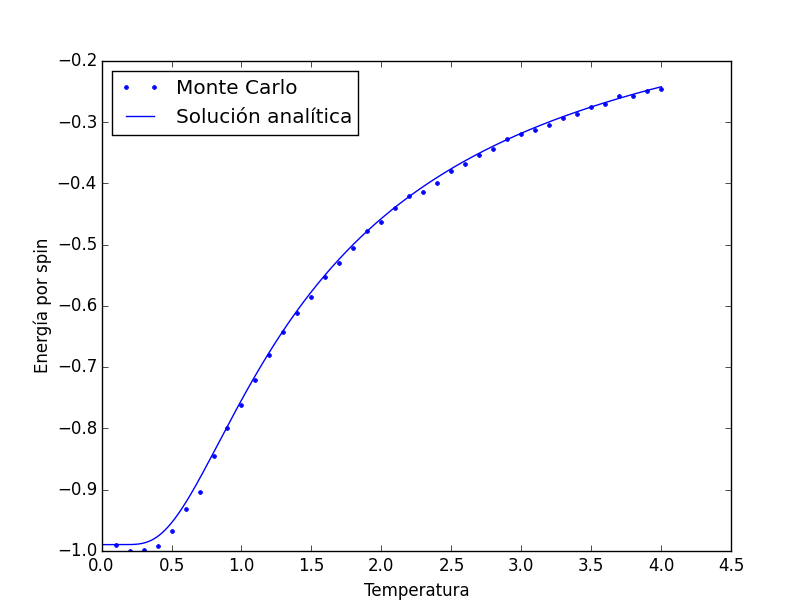
\includegraphics[width=\linewidth]{Ising.png}
\end{column}
\end{columns}
\end{frame}

\begin{frame}{Modelo de Ising en una dimensión}
\justifying
Consideremos una cadena de $N$ espines, donde cada sitio puede tomar dos valores:
\[
S_i = \pm 1.
\]

La energía del sistema, en ausencia de campo externo, es
\[
H(S_1,\ldots,S_N) = -J\sum_{i=1}^{N-1} S_i S_{i+1}.
\]

\begin{itemize}
    \item Si $J>0$, espines vecinos paralelos reducen la energía.
    \item El sistema favorece alineamiento: todos arriba o todos abajo.
    \item La temperatura compite contra esa tendencia al orden.
\end{itemize}

\begin{alertblock}{Interpretación}
Es un modelo extremadamente simple, pero ya captura la competencia entre \textbf{interacción} y \textbf{fluctuaciones térmicas}.
\end{alertblock}
\end{frame}

\begin{frame}{Observables en el modelo de Ising}
\small
Una vez generadas configuraciones con la distribución de equilibrio, podemos medir:

\begin{equation*}
E = -J\sum_{i=1}^{N-1} S_iS_{i+1},
\qquad
M = \sum_{i=1}^{N} S_i.
\end{equation*}

\begin{itemize}
    \item \textbf{Energía}: indica qué tan alineados están los espines vecinos.
    \item \textbf{Magnetización}: mide el balance global entre espines $+1$ y $-1$.
    \item \textbf{Promedios térmicos}: se obtienen promediando estas cantidades a lo largo de la simulación.
\end{itemize}

\begin{block}{Pregunta física}
¿Cómo cambia la energía media por espín cuando aumentamos la temperatura?
\end{block}
\end{frame}

\begin{frame}{Resultado analítico en una dimensión}
\justifying
El modelo de Ising 1D tiene solución exacta. Para una cadena abierta, la energía media es

\begin{equation*}
\langle H \rangle_\beta = -(N-1)J\tanh(\beta J).
\end{equation*}

Por lo tanto, la energía media \textbf{por enlace} o, aproximadamente, por espín para $N$ grande, es
\begin{equation*}
\frac{\langle H \rangle}{N} \approx -J\tanh(\beta J).
\end{equation*}

\begin{itemize}
    \item Si $T$ es baja, $\tanh(\beta J)\to 1$ y la energía se acerca a su mínimo.
    \item Si $T$ es alta, $\tanh(\beta J)\to 0$ y el sistema se desordena.
\end{itemize}

\begin{alertblock}{Importancia didáctica}
Tenemos un caso donde la simulación puede compararse directamente con una respuesta analítica exacta.
\end{alertblock}
\end{frame}

\begin{frame}[fragile]{Código base: paso Metropolis en Ising 1D}
\inputminted[firstline=12,lastline=24]{python}{ising1d.py}
\end{frame}

\begin{frame}{Cierre Clase 1}
\begin{itemize}
    \item Metropolis transforma una distribución complicada en una regla de aceptación simple.
    \item El modelo de Ising es un laboratorio ideal para conectar teoría estadística y simulación.
    \item En una dimensión, la energía promedio exacta nos sirve como prueba de validación numérica.
\end{itemize}
\end{frame}

\section{Clase 2}

\begin{frame}[plain]
\centering
\vfill
{\Huge \bfseries Clase 2}\\[0.4cm]
{\Large Laboratorio guiado: simulación, visualización y extensiones del modelo de Ising}
\vfill
\end{frame}

\begin{frame}{Objetivos de la Clase 2}
\begin{itemize}
    \item Implementar una simulación del modelo de Ising 1D para distintas temperaturas.
    \item Comparar resultados numéricos con la solución analítica de la energía promedio.
    \item Visualizar configuraciones de espines y discutir tiempo de equilibración.
    \item Explorar cómo cambia el problema al pasar al modelo de Ising 2D.
\end{itemize}
\end{frame}

\begin{frame}{Flujo de una simulación en la práctica}
\small
\begin{enumerate}
    \item Inicializar una cadena aleatoria de espines.
    \item Elegir una temperatura $T$.
    \item Repetir muchos pasos de Monte Carlo:
    \begin{itemize}
        \item elegir un espín al azar;
        \item proponer invertirlo;
        \item calcular $\Delta E$;
        \item aceptar o rechazar el cambio.
    \end{itemize}
    \item Descartar una etapa inicial de \textbf{equilibración}.
    \item Promediar energía y, si se desea, magnetización.
    \item Repetir para distintos valores de $T$.
\end{enumerate}

\begin{block}{Buena práctica}
Separar el código en funciones como \texttt{Energy()}, \texttt{step\_metropolis()} y \texttt{measure()} ayuda a depurar y extender el programa.
\end{block}
\end{frame}

\begin{frame}{Qué observar en los resultados}
\begin{columns}[T]
\begin{column}{0.55\textwidth}
\begin{itemize}
    \item A baja temperatura aparecen dominios largos y estados muy alineados.
    \item A alta temperatura la cadena se ve desordenada y fluctúa más.
    \item La energía media debería seguir la curva analítica dentro del error estadístico.
    \item El ruido disminuye al aumentar el número de pasos de Monte Carlo.
\end{itemize}
\end{column}
\begin{column}{0.45\textwidth}
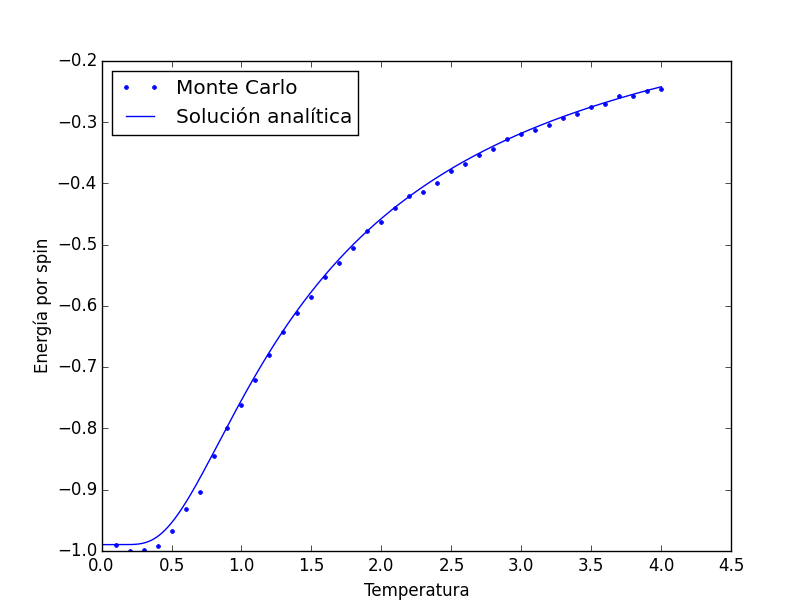
\includegraphics[width=\linewidth]{Ising.png}
\end{column}
\end{columns}
\end{frame}

\begin{frame}[fragile]{Código de apoyo: inicialización visual de espines}
\inputminted[firstline=45,lastline=55]{python}{spins_plot.py}
\end{frame}

\begin{frame}[fragile]{Código de apoyo: barrido en temperatura}
\inputminted[firstline=16,lastline=31]{python}{ising1d.py}
\end{frame}

\begin{frame}{Del caso 1D al caso 2D}
\justifying
En dos dimensiones, cada espín interactúa con más vecinos y el comportamiento
colectivo cambia de forma cualitativa. En particular, aparece una
\textbf{transición de fase} a temperatura crítica finita, algo que no ocurre en
el caso unidimensional sin campo externo.

\begin{itemize}
    \item En 2D la visualización de dominios es especialmente informativa.
    \item La magnetización se vuelve un observable central.
    \item El costo computacional crece y conviene pensar mejor la estructura del código.
\end{itemize}

\begin{alertblock}{Proyección}
El caso 2D es un excelente puente entre programación, física estadística y fenómenos emergentes.
\end{alertblock}
\end{frame}

\begin{frame}[fragile]{Extensión sugerida: vecinos y energía en Ising 2D}
\inputminted[firstline=13,lastline=27]{python}{ising2d.py}
\end{frame}

\begin{frame}[fragile]{Extensión sugerida: magnetización en Ising 2D}
\inputminted[firstline=36,lastline=54]{python}{ising2d.py}
\end{frame}

\begin{frame}{Actividades propuestas}
\begin{enumerate}
    \item \textbf{Validación 1D}: simular una cadena de $N=100$ espines entre $T=0.1$ y $T=4.0$.
    \item \textbf{Comparación}: graficar energía promedio por espín y superponer la curva analítica.
    \item \textbf{Equilibración}: repetir el experimento descartando distintos números de pasos iniciales.
    \item \textbf{Visualización}: guardar configuraciones típicas para una temperatura baja, media y alta.
    \item \textbf{Desafío}: adaptar el código para medir magnetización y explorar una red bidimensional.
\end{enumerate}

\begin{block}{Entregable sugerido}
Notebook o script con gráficos, breve discusión del error estadístico y comentario físico sobre el efecto de la temperatura.
\end{block}
\end{frame}

\begin{frame}{Preguntas guía para discutir en clase}
\begin{itemize}
    \item ¿Qué diferencias observamos entre el régimen ordenado y desordenado?
    \item ¿Cómo afecta el número de pasos a la estabilidad del promedio?
    \item ¿Por qué conviene descartar un tiempo inicial de equilibración?
    \item ¿Qué cambia al pasar de una cadena 1D a una red 2D con condiciones periódicas?
\end{itemize}
\end{frame}

\begin{frame}{Cierre de la semana}
\begin{itemize}
    \item Metropolis es uno de los algoritmos centrales de la física computacional.
    \item El modelo de Ising muestra cómo reglas locales simples producen comportamiento colectivo no trivial.
    \item La comparación entre teoría y simulación deja una base útil para temas posteriores del curso.
\end{itemize}
\end{frame}

\end{document}
